\documentclass[conference]{IEEEtran}
\IEEEoverridecommandlockouts
\usepackage[utf8]{inputenc}
\usepackage[T1]{fontenc}
\usepackage{lmodern}
\usepackage{amsmath}
\usepackage{graphicx}
\usepackage{booktabs}
\usepackage{xcolor}
\usepackage{url}
\usepackage[hidelinks]{hyperref}
\usepackage{cite}
\graphicspath{{figures/}}
% Generated by model/report.py from the results files. Do not edit by hand.
\newcommand{\BaselineTrivialMeanFullTwoOneTestRmse}{41.58}
\newcommand{\BaselineTrivialMeanFullTwoOneTestRmseStd}{0.00}
\newcommand{\BaselineTrivialMeanFullTwoOneTestMae}{36.98}
\newcommand{\BaselineTrivialMeanFullTwoOneTestNasa}{302.35}
\newcommand{\BaselineTrivialMeanFullTwoOneStatusAcc}{0.717}
\newcommand{\BaselineTrivialMeanFullTwoOneStatusAccPct}{71.7}
\newcommand{\BaselineTrivialMeanFullTwoOneStatusFOne}{0.278}
\newcommand{\BaselineTrivialMeanFullTwoOneCriticalRecall}{0.000}
\newcommand{\BaselineTrivialMeanFullTwoOneOfficialRmse}{41.97}
\newcommand{\BaselineTrivialMeanFullTwoOneNEstimators}{0}
\newcommand{\BaselineTrivialMeanFullTwoOneNSensors}{21}
\newcommand{\BaselineTrivialMeanFullTwoOneTrainSeconds}{0}
\newcommand{\BaselineRidgeFullTwoOneTestRmse}{18.78}
\newcommand{\BaselineRidgeFullTwoOneTestRmseStd}{0.00}
\newcommand{\BaselineRidgeFullTwoOneTestMae}{14.26}
\newcommand{\BaselineRidgeFullTwoOneTestNasa}{7.28}
\newcommand{\BaselineRidgeFullTwoOneStatusAcc}{0.850}
\newcommand{\BaselineRidgeFullTwoOneStatusAccPct}{85.0}
\newcommand{\BaselineRidgeFullTwoOneStatusFOne}{0.700}
\newcommand{\BaselineRidgeFullTwoOneCriticalRecall}{0.640}
\newcommand{\BaselineRidgeFullTwoOneOfficialRmse}{19.45}
\newcommand{\BaselineRidgeFullTwoOneNEstimators}{0}
\newcommand{\BaselineRidgeFullTwoOneNSensors}{21}
\newcommand{\BaselineRidgeFullTwoOneTrainSeconds}{0}
\newcommand{\BaselineTrivialMeanInformativeOneFiveTestRmse}{41.58}
\newcommand{\BaselineTrivialMeanInformativeOneFiveTestRmseStd}{0.00}
\newcommand{\BaselineTrivialMeanInformativeOneFiveTestMae}{36.98}
\newcommand{\BaselineTrivialMeanInformativeOneFiveTestNasa}{302.35}
\newcommand{\BaselineTrivialMeanInformativeOneFiveStatusAcc}{0.717}
\newcommand{\BaselineTrivialMeanInformativeOneFiveStatusAccPct}{71.7}
\newcommand{\BaselineTrivialMeanInformativeOneFiveStatusFOne}{0.278}
\newcommand{\BaselineTrivialMeanInformativeOneFiveCriticalRecall}{0.000}
\newcommand{\BaselineTrivialMeanInformativeOneFiveOfficialRmse}{41.97}
\newcommand{\BaselineTrivialMeanInformativeOneFiveNEstimators}{0}
\newcommand{\BaselineTrivialMeanInformativeOneFiveNSensors}{15}
\newcommand{\BaselineTrivialMeanInformativeOneFiveTrainSeconds}{0}
\newcommand{\BaselineRidgeInformativeOneFiveTestRmse}{19.01}
\newcommand{\BaselineRidgeInformativeOneFiveTestRmseStd}{0.00}
\newcommand{\BaselineRidgeInformativeOneFiveTestMae}{14.37}
\newcommand{\BaselineRidgeInformativeOneFiveTestNasa}{7.77}
\newcommand{\BaselineRidgeInformativeOneFiveStatusAcc}{0.850}
\newcommand{\BaselineRidgeInformativeOneFiveStatusAccPct}{85.0}
\newcommand{\BaselineRidgeInformativeOneFiveStatusFOne}{0.699}
\newcommand{\BaselineRidgeInformativeOneFiveCriticalRecall}{0.638}
\newcommand{\BaselineRidgeInformativeOneFiveOfficialRmse}{19.53}
\newcommand{\BaselineRidgeInformativeOneFiveNEstimators}{0}
\newcommand{\BaselineRidgeInformativeOneFiveNSensors}{15}
\newcommand{\BaselineRidgeInformativeOneFiveTrainSeconds}{0}
\newcommand{\BaselineTrivialMeanReducedEightTestRmse}{41.58}
\newcommand{\BaselineTrivialMeanReducedEightTestRmseStd}{0.00}
\newcommand{\BaselineTrivialMeanReducedEightTestMae}{36.98}
\newcommand{\BaselineTrivialMeanReducedEightTestNasa}{302.35}
\newcommand{\BaselineTrivialMeanReducedEightStatusAcc}{0.717}
\newcommand{\BaselineTrivialMeanReducedEightStatusAccPct}{71.7}
\newcommand{\BaselineTrivialMeanReducedEightStatusFOne}{0.278}
\newcommand{\BaselineTrivialMeanReducedEightCriticalRecall}{0.000}
\newcommand{\BaselineTrivialMeanReducedEightOfficialRmse}{41.97}
\newcommand{\BaselineTrivialMeanReducedEightNEstimators}{0}
\newcommand{\BaselineTrivialMeanReducedEightNSensors}{8}
\newcommand{\BaselineTrivialMeanReducedEightTrainSeconds}{0}
\newcommand{\BaselineRidgeReducedEightTestRmse}{20.86}
\newcommand{\BaselineRidgeReducedEightTestRmseStd}{0.00}
\newcommand{\BaselineRidgeReducedEightTestMae}{15.61}
\newcommand{\BaselineRidgeReducedEightTestNasa}{9.21}
\newcommand{\BaselineRidgeReducedEightStatusAcc}{0.849}
\newcommand{\BaselineRidgeReducedEightStatusAccPct}{84.9}
\newcommand{\BaselineRidgeReducedEightStatusFOne}{0.695}
\newcommand{\BaselineRidgeReducedEightCriticalRecall}{0.616}
\newcommand{\BaselineRidgeReducedEightOfficialRmse}{21.33}
\newcommand{\BaselineRidgeReducedEightNEstimators}{0}
\newcommand{\BaselineRidgeReducedEightNSensors}{8}
\newcommand{\BaselineRidgeReducedEightTrainSeconds}{0}
\newcommand{\MainGbrFullTwoOneTestRmse}{12.99}
\newcommand{\MainGbrFullTwoOneTestRmseStd}{0.07}
\newcommand{\MainGbrFullTwoOneTestMae}{9.40}
\newcommand{\MainGbrFullTwoOneTestNasa}{2.86}
\newcommand{\MainGbrFullTwoOneStatusAcc}{0.921}
\newcommand{\MainGbrFullTwoOneStatusAccPct}{92.1}
\newcommand{\MainGbrFullTwoOneStatusFOne}{0.845}
\newcommand{\MainGbrFullTwoOneCriticalRecall}{0.933}
\newcommand{\MainGbrFullTwoOneOfficialRmse}{13.22}
\newcommand{\MainGbrFullTwoOneNEstimators}{200}
\newcommand{\MainGbrFullTwoOneNSensors}{21}
\newcommand{\MainGbrFullTwoOneTrainSeconds}{245}
\newcommand{\MainGbrInformativeOneFiveTestRmse}{12.99}
\newcommand{\MainGbrInformativeOneFiveTestRmseStd}{0.07}
\newcommand{\MainGbrInformativeOneFiveTestMae}{9.40}
\newcommand{\MainGbrInformativeOneFiveTestNasa}{2.86}
\newcommand{\MainGbrInformativeOneFiveStatusAcc}{0.921}
\newcommand{\MainGbrInformativeOneFiveStatusAccPct}{92.1}
\newcommand{\MainGbrInformativeOneFiveStatusFOne}{0.845}
\newcommand{\MainGbrInformativeOneFiveCriticalRecall}{0.933}
\newcommand{\MainGbrInformativeOneFiveOfficialRmse}{13.22}
\newcommand{\MainGbrInformativeOneFiveNEstimators}{200}
\newcommand{\MainGbrInformativeOneFiveNSensors}{15}
\newcommand{\MainGbrInformativeOneFiveTrainSeconds}{255}
\newcommand{\MainGbrReducedEightTestRmse}{15.56}
\newcommand{\MainGbrReducedEightTestRmseStd}{0.06}
\newcommand{\MainGbrReducedEightTestMae}{11.15}
\newcommand{\MainGbrReducedEightTestNasa}{4.35}
\newcommand{\MainGbrReducedEightStatusAcc}{0.913}
\newcommand{\MainGbrReducedEightStatusAccPct}{91.3}
\newcommand{\MainGbrReducedEightStatusFOne}{0.832}
\newcommand{\MainGbrReducedEightCriticalRecall}{0.935}
\newcommand{\MainGbrReducedEightOfficialRmse}{15.35}
\newcommand{\MainGbrReducedEightNEstimators}{300}
\newcommand{\MainGbrReducedEightNSensors}{8}
\newcommand{\MainGbrReducedEightTrainSeconds}{136}
\newcommand{\PosthocGbrGreedyEightTestRmse}{13.88}
\newcommand{\PosthocGbrGreedyEightTestRmseStd}{0.12}
\newcommand{\PosthocGbrGreedyEightTestMae}{9.88}
\newcommand{\PosthocGbrGreedyEightTestNasa}{3.34}
\newcommand{\PosthocGbrGreedyEightStatusAcc}{0.918}
\newcommand{\PosthocGbrGreedyEightStatusAccPct}{91.8}
\newcommand{\PosthocGbrGreedyEightStatusFOne}{0.844}
\newcommand{\PosthocGbrGreedyEightCriticalRecall}{0.932}
\newcommand{\PosthocGbrGreedyEightOfficialRmse}{13.20}
\newcommand{\PosthocGbrGreedyEightNEstimators}{300}
\newcommand{\PosthocGbrGreedyEightNSensors}{8}
\newcommand{\PosthocGbrGreedyEightTrainSeconds}{115}
\newcommand{\PosthocGbrFullTwoOneWOneZeroTestRmse}{17.79}
\newcommand{\PosthocGbrFullTwoOneWOneZeroTestRmseStd}{0.04}
\newcommand{\PosthocGbrFullTwoOneWOneZeroTestMae}{12.61}
\newcommand{\PosthocGbrFullTwoOneWOneZeroTestNasa}{11.63}
\newcommand{\PosthocGbrFullTwoOneWOneZeroStatusAcc}{0.891}
\newcommand{\PosthocGbrFullTwoOneWOneZeroStatusAccPct}{89.1}
\newcommand{\PosthocGbrFullTwoOneWOneZeroStatusFOne}{0.794}
\newcommand{\PosthocGbrFullTwoOneWOneZeroCriticalRecall}{0.851}
\newcommand{\PosthocGbrFullTwoOneWOneZeroOfficialRmse}{18.13}
\newcommand{\PosthocGbrFullTwoOneWOneZeroNEstimators}{200}
\newcommand{\PosthocGbrFullTwoOneWOneZeroNSensors}{21}
\newcommand{\PosthocGbrFullTwoOneWOneZeroTrainSeconds}{184}
\newcommand{\PosthocGbrReducedEightWOneZeroTestRmse}{19.01}
\newcommand{\PosthocGbrReducedEightWOneZeroTestRmseStd}{0.04}
\newcommand{\PosthocGbrReducedEightWOneZeroTestMae}{14.24}
\newcommand{\PosthocGbrReducedEightWOneZeroTestNasa}{11.31}
\newcommand{\PosthocGbrReducedEightWOneZeroStatusAcc}{0.874}
\newcommand{\PosthocGbrReducedEightWOneZeroStatusAccPct}{87.4}
\newcommand{\PosthocGbrReducedEightWOneZeroStatusFOne}{0.749}
\newcommand{\PosthocGbrReducedEightWOneZeroCriticalRecall}{0.814}
\newcommand{\PosthocGbrReducedEightWOneZeroOfficialRmse}{19.71}
\newcommand{\PosthocGbrReducedEightWOneZeroNEstimators}{200}
\newcommand{\PosthocGbrReducedEightWOneZeroNSensors}{8}
\newcommand{\PosthocGbrReducedEightWOneZeroTrainSeconds}{108}
\newcommand{\PosthocGbrFullTwoOneWSixZeroTestRmse}{11.16}
\newcommand{\PosthocGbrFullTwoOneWSixZeroTestRmseStd}{0.11}
\newcommand{\PosthocGbrFullTwoOneWSixZeroTestMae}{8.07}
\newcommand{\PosthocGbrFullTwoOneWSixZeroTestNasa}{1.96}
\newcommand{\PosthocGbrFullTwoOneWSixZeroStatusAcc}{0.932}
\newcommand{\PosthocGbrFullTwoOneWSixZeroStatusAccPct}{93.2}
\newcommand{\PosthocGbrFullTwoOneWSixZeroStatusFOne}{0.880}
\newcommand{\PosthocGbrFullTwoOneWSixZeroCriticalRecall}{0.921}
\newcommand{\PosthocGbrFullTwoOneWSixZeroOfficialRmse}{12.67}
\newcommand{\PosthocGbrFullTwoOneWSixZeroNEstimators}{800}
\newcommand{\PosthocGbrFullTwoOneWSixZeroNSensors}{21}
\newcommand{\PosthocGbrFullTwoOneWSixZeroTrainSeconds}{201}
\newcommand{\PosthocGbrReducedEightWSixZeroTestRmse}{12.91}
\newcommand{\PosthocGbrReducedEightWSixZeroTestRmseStd}{0.01}
\newcommand{\PosthocGbrReducedEightWSixZeroTestMae}{9.35}
\newcommand{\PosthocGbrReducedEightWSixZeroTestNasa}{2.51}
\newcommand{\PosthocGbrReducedEightWSixZeroStatusAcc}{0.925}
\newcommand{\PosthocGbrReducedEightWSixZeroStatusAccPct}{92.5}
\newcommand{\PosthocGbrReducedEightWSixZeroStatusFOne}{0.871}
\newcommand{\PosthocGbrReducedEightWSixZeroCriticalRecall}{0.956}
\newcommand{\PosthocGbrReducedEightWSixZeroOfficialRmse}{14.07}
\newcommand{\PosthocGbrReducedEightWSixZeroNEstimators}{300}
\newcommand{\PosthocGbrReducedEightWSixZeroNSensors}{8}
\newcommand{\PosthocGbrReducedEightWSixZeroTrainSeconds}{124}
\newcommand{\PosthocGbrRandomEightZeroTestRmse}{15.58}
\newcommand{\PosthocGbrRandomEightZeroTestRmseStd}{0.06}
\newcommand{\PosthocGbrRandomEightZeroTestMae}{11.16}
\newcommand{\PosthocGbrRandomEightZeroTestNasa}{5.12}
\newcommand{\PosthocGbrRandomEightZeroStatusAcc}{0.903}
\newcommand{\PosthocGbrRandomEightZeroStatusAccPct}{90.3}
\newcommand{\PosthocGbrRandomEightZeroStatusFOne}{0.812}
\newcommand{\PosthocGbrRandomEightZeroCriticalRecall}{0.886}
\newcommand{\PosthocGbrRandomEightZeroOfficialRmse}{14.43}
\newcommand{\PosthocGbrRandomEightZeroNEstimators}{200}
\newcommand{\PosthocGbrRandomEightZeroNSensors}{8}
\newcommand{\PosthocGbrRandomEightZeroTrainSeconds}{107}
\newcommand{\PosthocGbrRandomEightOneTestRmse}{13.81}
\newcommand{\PosthocGbrRandomEightOneTestRmseStd}{0.08}
\newcommand{\PosthocGbrRandomEightOneTestMae}{9.88}
\newcommand{\PosthocGbrRandomEightOneTestNasa}{3.86}
\newcommand{\PosthocGbrRandomEightOneStatusAcc}{0.922}
\newcommand{\PosthocGbrRandomEightOneStatusAccPct}{92.2}
\newcommand{\PosthocGbrRandomEightOneStatusFOne}{0.854}
\newcommand{\PosthocGbrRandomEightOneCriticalRecall}{0.924}
\newcommand{\PosthocGbrRandomEightOneOfficialRmse}{14.52}
\newcommand{\PosthocGbrRandomEightOneNEstimators}{200}
\newcommand{\PosthocGbrRandomEightOneNSensors}{8}
\newcommand{\PosthocGbrRandomEightOneTrainSeconds}{116}
\newcommand{\PosthocGbrRandomEightTwoTestRmse}{14.81}
\newcommand{\PosthocGbrRandomEightTwoTestRmseStd}{0.05}
\newcommand{\PosthocGbrRandomEightTwoTestMae}{10.97}
\newcommand{\PosthocGbrRandomEightTwoTestNasa}{4.19}
\newcommand{\PosthocGbrRandomEightTwoStatusAcc}{0.902}
\newcommand{\PosthocGbrRandomEightTwoStatusAccPct}{90.2}
\newcommand{\PosthocGbrRandomEightTwoStatusFOne}{0.808}
\newcommand{\PosthocGbrRandomEightTwoCriticalRecall}{0.886}
\newcommand{\PosthocGbrRandomEightTwoOfficialRmse}{15.36}
\newcommand{\PosthocGbrRandomEightTwoNEstimators}{100}
\newcommand{\PosthocGbrRandomEightTwoNSensors}{8}
\newcommand{\PosthocGbrRandomEightTwoTrainSeconds}{103}
\newcommand{\PosthocGbrWorstEightTestRmse}{13.96}
\newcommand{\PosthocGbrWorstEightTestRmseStd}{0.07}
\newcommand{\PosthocGbrWorstEightTestMae}{10.05}
\newcommand{\PosthocGbrWorstEightTestNasa}{3.90}
\newcommand{\PosthocGbrWorstEightStatusAcc}{0.917}
\newcommand{\PosthocGbrWorstEightStatusAccPct}{91.7}
\newcommand{\PosthocGbrWorstEightStatusFOne}{0.843}
\newcommand{\PosthocGbrWorstEightCriticalRecall}{0.910}
\newcommand{\PosthocGbrWorstEightOfficialRmse}{14.08}
\newcommand{\PosthocGbrWorstEightNEstimators}{200}
\newcommand{\PosthocGbrWorstEightNSensors}{8}
\newcommand{\PosthocGbrWorstEightTrainSeconds}{5003}
\newcommand{\PosthocGbrFullTwoOneRowsplitTestRmse}{10.08}
\newcommand{\PosthocGbrFullTwoOneRowsplitTestRmseStd}{0.27}
\newcommand{\PosthocGbrFullTwoOneRowsplitTestMae}{7.06}
\newcommand{\PosthocGbrFullTwoOneRowsplitTestNasa}{1.63}
\newcommand{\PosthocGbrFullTwoOneRowsplitStatusAcc}{0.934}
\newcommand{\PosthocGbrFullTwoOneRowsplitStatusAccPct}{93.4}
\newcommand{\PosthocGbrFullTwoOneRowsplitStatusFOne}{0.884}
\newcommand{\PosthocGbrFullTwoOneRowsplitCriticalRecall}{0.921}
\newcommand{\PosthocGbrFullTwoOneRowsplitOfficialRmse}{13.54}
\newcommand{\PosthocGbrFullTwoOneRowsplitNEstimators}{200}
\newcommand{\PosthocGbrFullTwoOneRowsplitNSensors}{21}
\newcommand{\PosthocGbrFullTwoOneRowsplitTrainSeconds}{63}
\newcommand{\PosthocGbrFullTwoOneCapOneZeroZeroTestRmse}{8.42}
\newcommand{\PosthocGbrFullTwoOneCapOneZeroZeroTestRmseStd}{0.06}
\newcommand{\PosthocGbrFullTwoOneCapOneZeroZeroTestMae}{5.60}
\newcommand{\PosthocGbrFullTwoOneCapOneZeroZeroTestNasa}{1.14}
\newcommand{\PosthocGbrFullTwoOneCapOneZeroZeroStatusAcc}{0.923}
\newcommand{\PosthocGbrFullTwoOneCapOneZeroZeroStatusAccPct}{92.3}
\newcommand{\PosthocGbrFullTwoOneCapOneZeroZeroStatusFOne}{0.855}
\newcommand{\PosthocGbrFullTwoOneCapOneZeroZeroCriticalRecall}{0.930}
\newcommand{\PosthocGbrFullTwoOneCapOneZeroZeroOfficialRmse}{9.40}
\newcommand{\PosthocGbrFullTwoOneCapOneZeroZeroNEstimators}{200}
\newcommand{\PosthocGbrFullTwoOneCapOneZeroZeroNSensors}{21}
\newcommand{\PosthocGbrFullTwoOneCapOneZeroZeroTrainSeconds}{240}
\newcommand{\PosthocGbrReducedEightCapOneZeroZeroTestRmse}{10.26}
\newcommand{\PosthocGbrReducedEightCapOneZeroZeroTestRmseStd}{0.10}
\newcommand{\PosthocGbrReducedEightCapOneZeroZeroTestMae}{6.83}
\newcommand{\PosthocGbrReducedEightCapOneZeroZeroTestNasa}{1.57}
\newcommand{\PosthocGbrReducedEightCapOneZeroZeroStatusAcc}{0.919}
\newcommand{\PosthocGbrReducedEightCapOneZeroZeroStatusAccPct}{91.9}
\newcommand{\PosthocGbrReducedEightCapOneZeroZeroStatusFOne}{0.846}
\newcommand{\PosthocGbrReducedEightCapOneZeroZeroCriticalRecall}{0.933}
\newcommand{\PosthocGbrReducedEightCapOneZeroZeroOfficialRmse}{11.59}
\newcommand{\PosthocGbrReducedEightCapOneZeroZeroNEstimators}{400}
\newcommand{\PosthocGbrReducedEightCapOneZeroZeroNSensors}{8}
\newcommand{\PosthocGbrReducedEightCapOneZeroZeroTrainSeconds}{135}
\newcommand{\PosthocGbrFullTwoOneCapOneFiveZeroTestRmse}{19.14}
\newcommand{\PosthocGbrFullTwoOneCapOneFiveZeroTestRmseStd}{0.05}
\newcommand{\PosthocGbrFullTwoOneCapOneFiveZeroTestMae}{14.49}
\newcommand{\PosthocGbrFullTwoOneCapOneFiveZeroTestNasa}{8.50}
\newcommand{\PosthocGbrFullTwoOneCapOneFiveZeroStatusAcc}{0.912}
\newcommand{\PosthocGbrFullTwoOneCapOneFiveZeroStatusAccPct}{91.2}
\newcommand{\PosthocGbrFullTwoOneCapOneFiveZeroStatusFOne}{0.826}
\newcommand{\PosthocGbrFullTwoOneCapOneFiveZeroCriticalRecall}{0.926}
\newcommand{\PosthocGbrFullTwoOneCapOneFiveZeroOfficialRmse}{17.98}
\newcommand{\PosthocGbrFullTwoOneCapOneFiveZeroNEstimators}{300}
\newcommand{\PosthocGbrFullTwoOneCapOneFiveZeroNSensors}{21}
\newcommand{\PosthocGbrFullTwoOneCapOneFiveZeroTrainSeconds}{230}
\newcommand{\PosthocGbrReducedEightCapOneFiveZeroTestRmse}{21.35}
\newcommand{\PosthocGbrReducedEightCapOneFiveZeroTestRmseStd}{0.12}
\newcommand{\PosthocGbrReducedEightCapOneFiveZeroTestMae}{16.11}
\newcommand{\PosthocGbrReducedEightCapOneFiveZeroTestNasa}{12.82}
\newcommand{\PosthocGbrReducedEightCapOneFiveZeroStatusAcc}{0.909}
\newcommand{\PosthocGbrReducedEightCapOneFiveZeroStatusAccPct}{90.9}
\newcommand{\PosthocGbrReducedEightCapOneFiveZeroStatusFOne}{0.821}
\newcommand{\PosthocGbrReducedEightCapOneFiveZeroCriticalRecall}{0.919}
\newcommand{\PosthocGbrReducedEightCapOneFiveZeroOfficialRmse}{19.23}
\newcommand{\PosthocGbrReducedEightCapOneFiveZeroNEstimators}{200}
\newcommand{\PosthocGbrReducedEightCapOneFiveZeroNSensors}{8}
\newcommand{\PosthocGbrReducedEightCapOneFiveZeroTrainSeconds}{130}
\newcommand{\Margin}{1.0}
\newcommand{\HypGap}{2.57}
\newcommand{\HypGapMin}{2.49}
\newcommand{\HypGapMax}{2.68}
\newcommand{\HypHolds}{no}
\newcommand{\DeployedArm}{full21}
\newcommand{\TrivOverGbr}{3.2}
\newcommand{\GreedyEightGap}{0.89}
\newcommand{\WorstEightGap}{0.97}
\newcommand{\RandomEightTestRmse}{14.74}
\newcommand{\RandomEightTestRmseStd}{0.77}
\newcommand{\RandomEightGap}{1.75}
\newcommand{\RandomEightDraws}{3}
\newcommand{\GapWOneZero}{1.22}
\newcommand{\GapWSixZero}{1.75}
\newcommand{\GapCapOneZeroZero}{1.84}
\newcommand{\GapCapOneFiveZero}{2.21}
\newcommand{\WindowEffectFullTwoOne}{1.83}
\newcommand{\RowsplitRmse}{10.08}
\newcommand{\RowsplitOptimism}{2.91}
\newcommand{\RowsplitOptimismPct}{22}
\newcommand{\GreedyEightSensors}{8, 9, 11, 12, 13, 14, 17, 20}
\newcommand{\ReducedEightSensors}{2, 3, 4, 11, 15, 17, 20, 21}
\newcommand{\InformativeSensors}{2, 3, 4, 6, 7, 8, 9, 11, 12, 13, 14, 15, 17, 20, 21}
\newcommand{\ConstantSensors}{1, 5, 10, 16, 18, 19}
\newcommand{\BootFullTwoOneCiLow}{11.19}
\newcommand{\BootFullTwoOneCiHigh}{14.65}
\newcommand{\BootCiOverSeed}{26}
\newcommand{\BootDraws}{10000}
\newcommand{\BootReducedEightGapLow}{1.24}
\newcommand{\BootReducedEightGapHigh}{3.89}
\newcommand{\BootReducedEightBelowMarginPct}{1}
\newcommand{\BootGreedyEightGapLow}{$-$0.05}
\newcommand{\BootGreedyEightGapHigh}{1.96}
\newcommand{\BootGreedyEightBelowMarginPct}{62}
\newcommand{\BootWorstEightGapLow}{$-$0.28}
\newcommand{\BootWorstEightGapHigh}{2.14}
\newcommand{\BootWorstEightBelowMarginPct}{53}
\newcommand{\BootGreedyEightVsRanked}{$-$1.68}
\newcommand{\BootGreedyEightVsRankedLow}{$-$3.69}
\newcommand{\BootGreedyEightVsRankedHigh}{0.52}
\newcommand{\BootGreedyEightBetterThanRanked}{no}
\newcommand{\BootWorstEightVsRanked}{$-$1.60}
\newcommand{\BootWorstEightVsRankedLow}{$-$3.98}
\newcommand{\BootWorstEightVsRankedHigh}{0.82}
\newcommand{\BootWorstEightBetterThanRanked}{no}
\newcommand{\RedundancyReducedEight}{0.97}
\newcommand{\RedundancyWorstEight}{0.52}
\newcommand{\RedundancyGreedyEight}{0.62}
\newcommand{\RedundancyInformativeOneFive}{0.71}
\newcommand{\ConfigAuditVerdict}{recipe unchanged}
\newcommand{\ConfigAuditChanged}{deployment\_rule, onnx}
\newcommand{\ConfigAuditAffecting}{0}
\newcommand{\MainConfigHashes}{0b24782979f5 (full21); 838cd9be81f5 (informative15, reduced8)}
\newcommand{\NMainConfigHashes}{2}
\newcommand{\RandomEightBestGap}{0.83}
\newcommand{\RandomEightWorstGap}{2.60}
\newcommand{\SplitTrain}{70}
\newcommand{\SplitVal}{15}
\newcommand{\SplitTest}{15}
\newcommand{\CfgLearningRate}{0.05}
\newcommand{\CfgMaxDepth}{4}
\newcommand{\CfgSubsample}{0.8}
\newcommand{\CfgGridMin}{100}
\newcommand{\CfgGridMax}{800}
\newcommand{\CfgFeaturesFull}{63}
\newcommand{\CfgParityTolExp}{-3}
\newcommand{\CfgFeatureTolExp}{-6}
\newcommand{\AlertWarningBelow}{60}
\newcommand{\AlertCriticalBelow}{30}
\newcommand{\AlertTrendWindow}{30}
\newcommand{\AlertTrendSlope}{$-$2.0}
\newcommand{\AlertTrendClearSlope}{$-$1.5}
\newcommand{\AlertMinWindowRows}{30}
\newcommand{\AlertCloseAfter}{5}
\newcommand{\AlertHysteresis}{10}
\newcommand{\ParityRows}{300}
\newcommand{\OriginalTrendDrop}{20}
\newcommand{\OriginalTrendWindow}{10}
\newcommand{\NRunsTotal}{57}
\newcommand{\NRunsMain}{9}
\newcommand{\NRunsPosthoc}{42}
\newcommand{\ConfigHash}{0b24782979f5}
\newcommand{\Window}{30}
\newcommand{\LabelCap}{125}
\newcommand{\NSeeds}{3}
\newcommand{\EdaRows}{20631}
\newcommand{\EdaEngines}{100}
\newcommand{\EdaLifeMin}{128}
\newcommand{\EdaLifeMax}{362}
\newcommand{\EdaLifeMedian}{199}
\newcommand{\EdaShareRowsAboveCap}{38.9}
\newcommand{\AuditConstSplits}{0}
\newcommand{\AuditImportanceOutsidePct}{19.5}
\newcommand{\AuditTopOutside}{9, 12, 14, 7}
\newcommand{\AlertReplayValEngines}{15}
\newcommand{\AlertReplayValEnginesPassing}{15}
\newcommand{\AlertReplayValAlertsTotal}{30}
\newcommand{\AlertReplayValMeanTrueRulAtWarning}{56.7}
\newcommand{\AlertReplayValMinTrueRulAtWarning}{38}
\newcommand{\AlertReplayValMeanTrueRulAtCritical}{29.0}
\newcommand{\AlertReplayValMinTrueRulAtCritical}{19}
\newcommand{\AlertReplayTestEngines}{15}
\newcommand{\AlertReplayTestEnginesPassing}{15}
\newcommand{\AlertReplayTestAlertsTotal}{30}
\newcommand{\AlertReplayTestMeanTrueRulAtWarning}{54.5}
\newcommand{\AlertReplayTestMinTrueRulAtWarning}{40}
\newcommand{\AlertReplayTestMeanTrueRulAtCritical}{31.7}
\newcommand{\AlertReplayTestMinTrueRulAtCritical}{21}
\newcommand{\AlertOriginalPass}{2}
\newcommand{\AlertOriginalAlerts}{59}
\newcommand{\AlertChosenPass}{15}
\newcommand{\RestartFileRows}{20631}
\newcommand{\RestartReadingsRows}{20631}
\newcommand{\RestartHealthScoresRows}{20631}
\newcommand{\RestartMachinesScoredExactlyOneToLife}{100}
\newcommand{\RestartMachines}{100}
\newcommand{\RestartRedeliveredAndIgnoredAsLate}{2}
\newcommand{\RestartFinalConsumerLag}{0}
\newcommand{\RestartMachinesWithAlertsDifferentFromUninterruptedRun}{0}
\newcommand{\RestartMachinesWithRepeatedAlertOfOneSeverity}{4}
\newcommand{\RestartMaxDiff}{9e$-$05}
\newcommand{\RestartSecondsDown}{24.5}
\newcommand{\RestartPeakLag}{11175}
\newcommand{\RestartReadingsWhileDown}{6585}
\newcommand{\RestartPassed}{yes}
\newcommand{\AllEnginesAlertPass}{96}
\newcommand{\EaTestRows}{3183}
\newcommand{\EaMisclassifiedRows}{248}
\newcommand{\EaInspected}{35}
\newcommand{\EaAmbiguous}{3}
\newcommand{\EaMislabeled}{0}
\newcommand{\EaModel}{32}
\newcommand{\EaTopConfusionRows}{135}
\newcommand{\EaSecondConfusionRows}{58}
\newcommand{\EaHealthyAsCriticalRows}{0}
\newcommand{\EaCriticalAsHealthyRows}{0}
\newcommand{\EaMisclassifiedPct}{7.8}
\newcommand{\EaSmallErrorPct}{27}
\newcommand{\EaPatternLagging}{16}
\newcommand{\EaPatternJitter}{8}
\newcommand{\EaPatternEarly}{8}
\newcommand{\EaPatternPlateau}{2}
\newcommand{\EaPatternBoundary}{1}
\newcommand{\LtBeforeRps}{4138}
\newcommand{\LtBeforePFiveZero}{9.8}
\newcommand{\LtBeforePNineFive}{22.8}
\newcommand{\LtBeforePNineNine}{37.5}
\newcommand{\LtBeforeVus}{50}
\newcommand{\LtBeforeBatch}{1}
\newcommand{\LtBeforePoolPending}{30.4}
\newcommand{\LtBeforeDurationS}{60}
\newcommand{\LtBeforePoolPendingMax}{40}
\newcommand{\LtBeforeCpuPct}{41}
\newcommand{\LtBeforeProcessingMs}{0.97}
\newcommand{\LtBeforeInferenceMs}{0.13}
\newcommand{\LtBeforeDrainS}{0.3}
\newcommand{\LtBeforeScored}{239915}
\newcommand{\LtBeforeProcessedRps}{4115}
\newcommand{\LtBeforeRpsStd}{133}
\newcommand{\LtBeforePNineFiveStd}{0.4}
\newcommand{\LtBeforePNineNineStd}{1.7}
\newcommand{\LtBeforeRuns}{3}
\newcommand{\LtBeforePool}{10}
\newcommand{\LtAfterRps}{4318}
\newcommand{\LtAfterPFiveZero}{7.9}
\newcommand{\LtAfterPNineFive}{22.7}
\newcommand{\LtAfterPNineNine}{38.6}
\newcommand{\LtAfterVus}{50}
\newcommand{\LtAfterBatch}{1}
\newcommand{\LtAfterPoolPending}{1.3}
\newcommand{\LtAfterDurationS}{60}
\newcommand{\LtAfterPoolPendingMax}{10}
\newcommand{\LtAfterCpuPct}{41}
\newcommand{\LtAfterProcessingMs}{2.70}
\newcommand{\LtAfterInferenceMs}{0.14}
\newcommand{\LtAfterDrainS}{0.3}
\newcommand{\LtAfterScored}{235615}
\newcommand{\LtAfterProcessedRps}{4297}
\newcommand{\LtAfterRpsStd}{382}
\newcommand{\LtAfterPNineFiveStd}{1.9}
\newcommand{\LtAfterPNineNineStd}{4.6}
\newcommand{\LtAfterRuns}{3}
\newcommand{\LtAfterPool}{40}
\newcommand{\LtAfterCacheRps}{4550}
\newcommand{\LtAfterCachePFiveZero}{7.5}
\newcommand{\LtAfterCachePNineFive}{21.9}
\newcommand{\LtAfterCachePNineNine}{38.1}
\newcommand{\LtAfterCacheVus}{50}
\newcommand{\LtAfterCacheBatch}{1}
\newcommand{\LtAfterCachePoolPending}{1.3}
\newcommand{\LtAfterCacheDurationS}{60}
\newcommand{\LtAfterCachePoolPendingMax}{10}
\newcommand{\LtAfterCacheCpuPct}{40}
\newcommand{\LtAfterCacheProcessingMs}{2.86}
\newcommand{\LtAfterCacheInferenceMs}{0.14}
\newcommand{\LtAfterCacheDrainS}{0.3}
\newcommand{\LtAfterCacheScored}{245086}
\newcommand{\LtAfterCacheProcessedRps}{4528}
\newcommand{\LtAfterCacheRpsStd}{516}
\newcommand{\LtAfterCachePNineFiveStd}{2.5}
\newcommand{\LtAfterCachePNineNineStd}{6.3}
\newcommand{\LtAfterCacheRuns}{3}
\newcommand{\LtAfterCachePool}{40}
\newcommand{\LtKafkaRps}{4036}
\newcommand{\LtKafkaPFiveZero}{8.5}
\newcommand{\LtKafkaPNineFive}{24.3}
\newcommand{\LtKafkaPNineNine}{41.4}
\newcommand{\LtKafkaVus}{50}
\newcommand{\LtKafkaBatch}{1}
\newcommand{\LtKafkaPoolPending}{3.6}
\newcommand{\LtKafkaDurationS}{60}
\newcommand{\LtKafkaPoolPendingMax}{15}
\newcommand{\LtKafkaCpuPct}{38}
\newcommand{\LtKafkaProcessingMs}{1.64}
\newcommand{\LtKafkaInferenceMs}{0.14}
\newcommand{\LtKafkaDrainS}{64.9}
\newcommand{\LtKafkaScored}{214004}
\newcommand{\LtKafkaProcessedRps}{1938}
\newcommand{\LtKafkaRpsStd}{456}
\newcommand{\LtKafkaPNineFiveStd}{2.1}
\newcommand{\LtKafkaPNineNineStd}{5.9}
\newcommand{\LtKafkaRuns}{3}
\newcommand{\LtKafkaPool}{40}
\newcommand{\LtGainPct}{4}
\newcommand{\LtPoolGainMin}{$-$5}
\newcommand{\LtPoolGainMax}{10}
\newcommand{\LtPoolGainPositive}{2}
\newcommand{\LtPoolGainBlocks}{3}
\newcommand{\LtCacheGainMin}{3}
\newcommand{\LtCacheGainMax}{9}
\newcommand{\LtCacheGainPositive}{3}
\newcommand{\LtCacheGainBlocks}{3}
\newcommand{\LtTotalGainMin}{$-$2}
\newcommand{\LtTotalGainMax}{20}
\newcommand{\LtTotalGainPositive}{2}
\newcommand{\LtTotalGainBlocks}{3}
\newcommand{\LtPoolWaitsAllRunsMaxAfter}{4.4}
\newcommand{\LtPoolWaitsAllRunsMinBefore}{29.2}
\newcommand{\LtCacheGainPct}{5}
\newcommand{\LtTotalGainPct}{10}
\newcommand{\LtBestLabel}{after-cache}
\newcommand{\LtBestRps}{4550}
\newcommand{\LtBestPNineFive}{21.9}
\newcommand{\LtBestPNineNine}{38.1}
\newcommand{\JavaUsPerPrediction}{69.5}
\newcommand{\JavaPredictionsTimed}{5000}
\newcommand{\CoverageProcessingAlerts}{92.1}
\newcommand{\CoverageOverall}{91.6}
\newcommand{\CoverageRoot}{33.3}
\newcommand{\CoverageAlerts}{92.9}
\newcommand{\CoverageConfig}{96.6}
\newcommand{\CoverageIngest}{91.0}
\newcommand{\CoverageMachines}{91.1}
\newcommand{\CoverageModel}{93.9}
\newcommand{\CoverageProcessing}{91.5}
\newcommand{\CoverageQuery}{91.0}
\newcommand{\CoverageStream}{86.5}
\newcommand{\TestsJava}{58}
\newcommand{\TestsJavaFailed}{0}
\newcommand{\TestsPython}{16}
\newcommand{\TestsPythonFailed}{0}
\newcommand{\TestsPythonSkipped}{0}

\newcommand{\pmsd}[2]{#1\,$\pm$\,#2}
\hyphenation{Kafka Postgre-SQL Micro-meter}

\begin{document}

\title{Fewer Sensors, or the Wrong Ones?\\A Pre-registered Test of Sensor Reduction\\in a Real-Time Equipment Monitoring Service}

\author{\IEEEauthorblockN{Naren Kaarthik}
\IEEEauthorblockA{\textit{equipment-health-monitor} \\
\url{https://github.com/Narenkaarthik/equipment-health-monitor}}}

\maketitle

\begin{abstract}
We build a production-style monitoring service that ingests turbofan sensor readings as a stream, keeps a
sliding window per machine, predicts remaining useful life (RUL) with an in-process ONNX model, and raises
de-duplicated alerts. On top of it we ask whether the model can run on 8 of the 21 sensors without losing
accuracy. The test is pre-registered as non-inferiority with a margin of \Margin{} cycle of RMSE on held-out
engines of NASA C-MAPSS FD001, a simulated run-to-failure dataset. With the pre-registered ranking rule, the
answer is no: 8 ranked sensors are \HypGap{} cycles worse than all 21 (\MainGbrFullTwoOneTestRmse{} cycles RMSE).
Post hoc ablations show that the ranking, not the number 8, is what failed: random 8-sensor subsets do better on
average, and 8 sensors chosen by forward selection on validation engines come within \GreedyEightGap{} cycles.
A window-length ablation moves the error by about as much as the sensor reduction does, so the main result
holds only under its recipe. The service passes a kill-and-restart test with no lost or doubled reading and
alerts identical to an uninterrupted run, and opens exactly one WARNING and one CRITICAL alert on
\AlertReplayTestEnginesPassing{} of \AlertReplayTestEngines{} held-out engines replayed to failure.
\end{abstract}

\begin{IEEEkeywords}
predictive maintenance, remaining useful life, stream processing, pre-registration, ONNX, Kafka
\end{IEEEkeywords}

\section{Introduction}
Predictive-maintenance prototypes tend to be notebooks: a model and a score, with no stream, no state and no
failure handling. This work builds the system around the model and uses it to answer one engineering
question that matters for deployment: every sensor costs hardware, wiring and a failure mode, so can the
service run on fewer of them?

We make three contributions. First, a monitoring service in Java with a measured data path: ingest,
sliding-window features computed in $O(1)$ per reading, in-process ONNX scoring checked against Python, an
alert engine with explicit open, stay-open and close semantics, and Kafka between ingest and processing.
Second, a pre-registered sensor-reduction experiment with a frozen engine-level split, three seeds per arm,
validation-only model selection and a single read of the test split per run. Third, a post hoc analysis that
separates the idea (fewer sensors) from the recipe (which sensors, which window), reported as such.

\section{Data and setup}
NASA C-MAPSS FD001~\cite{saxena2008} simulates \EdaEngines{} turbofan engines from healthy to failure under one
operating condition and one fault mode; it is a physics-based benchmark, not field data. The training file
has \EdaRows{} rows of 21 sensors and three settings; engine life ranges from \EdaLifeMin{} to \EdaLifeMax{}
cycles (median \EdaLifeMedian{}). Sensors \ConstantSensors{} are constant.

\textbf{Split.} Engines are groups: \SplitTrain{} train, \SplitVal{} validation and \SplitTest{} test engines, frozen in a JSON
file with a test that fails if any engine appears in two splits. The official truncated test set is scored as a
secondary number comparable with the literature.

\textbf{Label and features.} RUL is capped at \LabelCap{} cycles, the usual convention for this
dataset~\cite{heimes2008}; \EdaShareRowsAboveCap{}\% of training rows are above the cap. For each sensor,
the mean, population standard deviation and least-squares slope over the last \Window{} readings form the
features (\CfgFeaturesFull{} for all sensors).

\textbf{Model.} Gradient-boosted regression trees (learning rate \CfgLearningRate{}, depth \CfgMaxDepth{},
subsample \CfgSubsample{}). The number of trees is chosen per arm from a grid of \CfgGridMin{} to \CfgGridMax{} by the lowest mean validation RMSE over the three seeds; the test split is
read once per finished run at the chosen size.

\section{The service}
\begin{figure}[t]
\centering
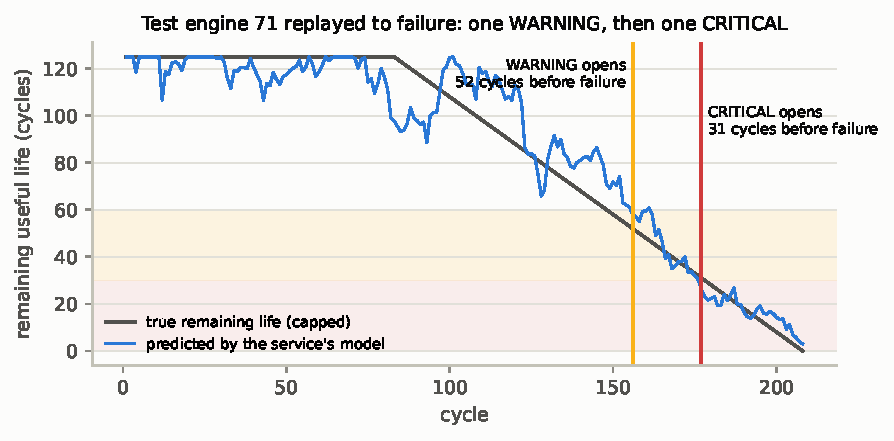
\includegraphics[width=\columnwidth]{alert_timeline.pdf}
\caption{A held-out engine replayed through the service to failure. The model's prediction follows the true
(capped) remaining life; one WARNING and one CRITICAL open, in that order, and neither repeats.}
\label{fig:timeline}
\end{figure}

A replayer streams each engine's rows in cycle order to an ingest API that validates a reading or a batch and
inserts it with \texttt{ON CONFLICT DO NOTHING} on the key (machine, cycle), so a repeated post is a no-op.
In the stage-5 configuration ingest publishes each reading to a Kafka topic keyed by machine id, so one machine's
readings stay ordered~\cite{kreps2011}, and returns once the broker acknowledges. A processor keeps one window
per machine. Running sums give the mean, variance and slope in $O(1)$ per reading; Java and Python agree within
$10^{\CfgFeatureTolExp}$ on a fixture. The cycle number is the machine's clock: late readings are ignored and gaps are tolerated.
The window is saved to Redis after the score and alerts are written, so a crash before the save leads to a
redelivery that is scored again idempotently. The model runs in-process with ONNX Runtime; on \ParityRows{} real
test rows Java and Python agree within $10^{\CfgParityTolExp}$ cycles, at \JavaUsPerPrediction{}\,\textmu s per prediction.

The alert engine has two rules. A threshold rule opens WARNING below \AlertWarningBelow{} and CRITICAL below
\AlertCriticalBelow{} predicted cycles. A trend rule opens WARNING when the least-squares slope of the prediction
over \AlertTrendWindow{} readings is below \AlertTrendSlope{} cycles per reading. An alert opens once per machine
and severity, stays open while any of its conditions holds, and closes after \AlertCloseAfter{} consecutive clear
readings, with \AlertHysteresis{} cycles of hysteresis on thresholds. No alert opens before the feature window
holds \AlertMinWindowRows{} readings. PostgreSQL stores readings, scores and alerts; the hot window lives in Redis,
much as Gorilla keeps recent data in memory~\cite{pelkonen2015}. Fig.~\ref{fig:timeline} shows one held-out engine.

\section{Pre-registered experiment}
\textbf{Hypothesis.} H1: the 8 sensors ranked highest by absolute Spearman correlation between their window mean
and RUL on the training engines (sensors \ReducedEightSensors{}) are non-inferior to all 21 sensors: the
mean test RMSE gap is below \Margin{} cycle. A third arm keeps the 15 informative (non-constant) sensors.
The recipe, the hypothesis and a deployment rule (ship the 8-sensor model only if H1 holds) were committed
before the first main result.

\begin{table*}[t]
\centering
\caption{Pre-registered comparison on \SplitTest{} held-out engines (mean $\pm$ std over seeds; baselines are deterministic).}
\label{tab:main}
\footnotesize
\setlength{\tabcolsep}{4pt}
\resizebox{\textwidth}{!}{\begin{tabular}{lrrrrrrrr}
\toprule
Method & Seeds & Test RMSE & Test MAE & NASA score & Status acc. & Macro-F1 & CRITICAL recall & Official RMSE \\
\midrule
trivial (train mean), all 21 sensors & 1 & 41.58 $\pm$ 0.00 & 36.98 $\pm$ 0.00 & 302.35 $\pm$ 0.00 & 0.717 & 0.278 & 0.000 & 41.97 $\pm$ 0.00 \\
ridge regression, all 21 sensors & 1 & 18.78 $\pm$ 0.00 & 14.26 $\pm$ 0.00 & 7.28 $\pm$ 0.00 & 0.850 & 0.700 & 0.640 & 19.45 $\pm$ 0.00 \\
ridge regression, 8 ranked sensors & 1 & 20.86 $\pm$ 0.00 & 15.61 $\pm$ 0.00 & 9.21 $\pm$ 0.00 & 0.849 & 0.695 & 0.616 & 21.33 $\pm$ 0.00 \\
gradient boosting, all 21 sensors & 3 & 12.99 $\pm$ 0.07 & 9.40 $\pm$ 0.09 & 2.86 $\pm$ 0.04 & 0.921 & 0.845 & 0.933 & 13.22 $\pm$ 0.12 \\
gradient boosting, 15 informative sensors & 3 & 12.99 $\pm$ 0.07 & 9.40 $\pm$ 0.09 & 2.86 $\pm$ 0.04 & 0.921 & 0.845 & 0.933 & 13.22 $\pm$ 0.12 \\
gradient boosting, 8 ranked sensors & 3 & 15.56 $\pm$ 0.06 & 11.15 $\pm$ 0.07 & 4.35 $\pm$ 0.07 & 0.913 & 0.832 & 0.935 & 15.35 $\pm$ 0.27 \\
\bottomrule
\end{tabular}
}
\end{table*}

\textbf{Result.} Table~\ref{tab:main}. All 21 sensors give \pmsd{\MainGbrFullTwoOneTestRmse}{\MainGbrFullTwoOneTestRmseStd}
cycles RMSE, \TrivOverGbr{} times better than predicting the training mean. The 8 ranked sensors give
\pmsd{\MainGbrReducedEightTestRmse}{\MainGbrReducedEightTestRmseStd}: a gap of \HypGap{} cycles, between
\HypGapMin{} and \HypGapMax{} when paired by seed. \textbf{H1 is rejected}, and the service ships the 21-sensor model.
The 15-sensor arm is identical to the 21-sensor arm: no tree splits on a constant sensor (\AuditConstSplits{} splits).
Status accuracy is not the headline because the classes are imbalanced: the trivial model scores
\BaselineTrivialMeanFullTwoOneStatusAccPct{}\% accuracy while catching no CRITICAL machine.

\textbf{Bug audit before the write-up.} The recomputed test errors match the results file for all nine
checkpoints, each checkpoint holds the arm, seed and feature count its name claims, and the 8-sensor
columns equal features rebuilt from scratch.

\section{Post hoc analysis}
Everything in this section was designed after the main result and is labelled post hoc. Each setting
uses the same model, grid, selection rule and three seeds.

\begin{figure}[t]
\centering
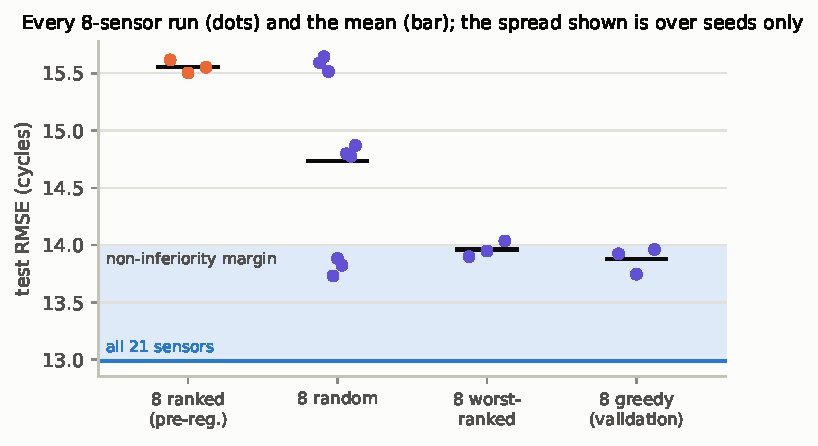
\includegraphics[width=\columnwidth]{which_eight.pdf}
\caption{Test RMSE of every 8-sensor run. The shaded band is the non-inferiority margin above the 21-sensor model.}
\label{fig:which8}
\end{figure}

\begin{table}[t]
\centering
\caption{Which 8 sensors (post hoc except the first two rows).}
\label{tab:which8}
\scriptsize
\setlength{\tabcolsep}{2.5pt}
\resizebox{\columnwidth}{!}{\begin{tabular}{llrrcl}
\toprule
Sensor set & Chosen by & Test RMSE & Gap to 21 & Within 1.0 & Phase \\
\midrule
all 21 sensors & all & 12.99 $\pm$ 0.07 & 0.00 &  & pre-registered \\
8 ranked sensors & pre-registered ranking (train) & 15.56 $\pm$ 0.06 & 2.57 & no & pre-registered \\
8 sensors, greedy on validation & forward selection (validation) & 13.88 $\pm$ 0.12 & 0.89 & yes & post hoc \\
8 random sensors (3 draws) & random & 14.74 $\pm$ 0.77 & 1.75 & no & post hoc \\
8 lowest-ranked sensors & bottom of the ranking & 13.96 $\pm$ 0.07 & 0.97 & yes & post hoc \\
\bottomrule
\end{tabular}
}
\end{table}

\textbf{Which 8, not how many.} The full model puts \AuditImportanceOutsidePct{}\% of its importance on sensors
\AuditTopOutside{}, which the ranking left out. Ranking each sensor alone selects sensors that move together:
the mean absolute correlation between the window means of the 8 ranked sensors is \RedundancyReducedEight{},
against \RedundancyWorstEight{} for the 8 lowest-ranked ones. Random 8-sensor subsets average
\RandomEightTestRmse{} cycles over \RandomEightDraws{} draws, better than the ranking. The 8 lowest-ranked
sensors give \PosthocGbrWorstEightTestRmse{}, inside the margin by a hair that three seeds cannot
resolve. Forward selection on the validation engines picks sensors \GreedyEightSensors{} and comes within
\GreedyEightGap{} cycles of the full model (Table~\ref{tab:which8}, Fig.~\ref{fig:which8}). Fewer sensors can
be enough; a univariate ranking is the wrong way to choose them.

\begin{figure}[t]
\centering
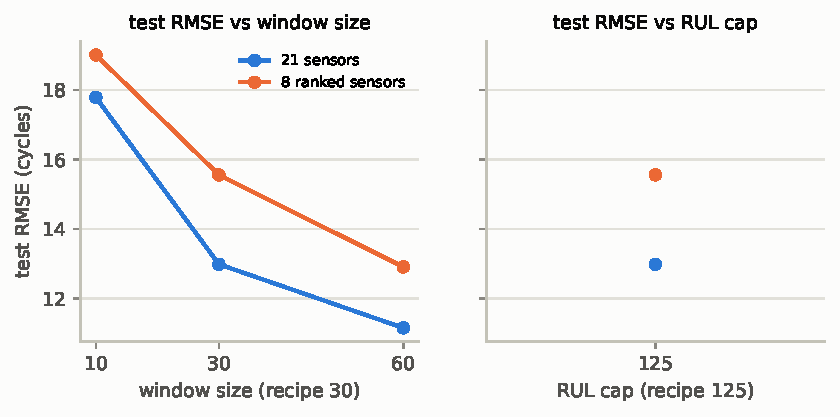
\includegraphics[width=\columnwidth]{recipe_sensitivity.pdf}
\caption{Test RMSE of the 21- and 8-sensor models as the window length and the RUL cap change (post hoc).}
\label{fig:recipe}
\end{figure}

\textbf{The recipe is as large as the effect.} The gap between 8 ranked and 21 sensors is \GapWOneZero{}
cycles with a 10-reading window and \GapWSixZero{} with a 60-reading window, against \HypGap{} at the
pre-registered \Window{} (Fig.~\ref{fig:recipe}). Moving the 21-sensor model from 30 to 60 readings improves it by
\WindowEffectFullTwoOne{} cycles, about the size of the sensor effect itself. The rejection holds in every
setting, but its size depends on the recipe; the main result should be read as conditional on it.

\textbf{The methodological gap.} Splitting rows at random, so that one engine's cycles fall on both sides,
reports \RowsplitRmse{} cycles RMSE for the same model, \RowsplitOptimismPct{}\% better than the
engine-level split. All of that is leak.

\section{Operational validation}
\textbf{Alerts.} The trend rule first specified, an end-to-end drop of more than \OriginalTrendDrop{} cycles over
\OriginalTrendWindow{} readings,
fired on the model's reading-to-reading jitter. It passed the one-WARNING-then-one-CRITICAL check on only
\AlertOriginalPass{} of \SplitVal{} validation engines. A Python simulator of the alert engine, cross-checked against the
service on every engine, found a Java bug on the way: after a restart the first score was counted twice. The
slope rule with a warm-up was designed on validation only (\AlertChosenPass{} of \SplitVal{}) and then checked once on the
test engines: \AlertReplayTestEnginesPassing{} of \AlertReplayTestEngines{} pass. CRITICAL opens on average
\AlertReplayTestMeanTrueRulAtCritical{} true cycles before failure, and never fewer than
\AlertReplayTestMinTrueRulAtCritical{}.

\textbf{Kill and restart.} Ingest and processor run as separate processes. The processor is killed mid-stream
with no shutdown hook and restarted \RestartSecondsDown{}\,s later, while ingest keeps accepting
(\RestartReadingsWhileDown{} readings arrive meanwhile). All \RestartFileRows{} readings are stored and scored
exactly once. Every score equals an uninterrupted run (maximum difference \RestartMaxDiff{}), every machine's
alerts are identical to an uninterrupted run, and \RestartRedeliveredAndIgnoredAsLate{} redelivered messages are
ignored as late.

\textbf{Throughput.} k6 posts one reading per request from \LtBeforeVus{} virtual users for \LtBeforeDurationS{}\,s, with every
component on one laptop (Table~\ref{tab:load}). The baseline sustained \LtBeforeRps{} readings per second at
p95 \LtBeforePNineFive{}\,ms. Sampled metrics located the first bottleneck: on average \LtBeforePoolPending{} requests waited
for one of \LtBeforePool{} database connections while CPU stayed at \LtBeforeCpuPct{}\%. A pool of \LtAfterPool{}
raised throughput by \LtGainPct{}\% to \LtAfterRps{} readings per second (p95 \LtAfterPNineFive{}\,ms, p99
\LtAfterPNineNine{}\,ms). Contention then moved to the database writes: processing time per reading rose from
\LtBeforeProcessingMs{} to \LtAfterProcessingMs{}\,ms. With the Kafka pipeline, ingest was not faster
(\LtKafkaRps{} readings per second), because each request waits for the broker's acknowledgement. Six consumer
threads processed \LtKafkaProcessedRps{} readings per second and drained the backlog \LtKafkaDrainS{}\,s after the load
stopped. Kafka buys isolation and durability here, not speed.

\begin{table}[t]
\centering
\caption{Load test of \texttt{POST /api/readings} (\LtBeforeDurationS{}\,s, one laptop).}
\label{tab:load}
\scriptsize
\setlength{\tabcolsep}{2.5pt}
\resizebox{\columnwidth}{!}{\begin{tabular}{llrrrrrr}
\toprule
Run & Pipeline & Repeats & Readings/s & p50 ms & p95 ms & p99 ms & Pool waits \\
\midrule
before & direct & 3 & 4138 $\pm$ 133 & 9.79 & 22.8 $\pm$ 0.4 & 37.5 $\pm$ 1.7 & 30.40 \\
after & direct & 3 & 4318 $\pm$ 382 & 7.90 & 22.7 $\pm$ 1.9 & 38.6 $\pm$ 4.6 & 1.35 \\
after-cache & direct & 3 & 4550 $\pm$ 516 & 7.48 & 21.9 $\pm$ 2.5 & 38.1 $\pm$ 6.3 & 1.26 \\
kafka & kafka & 3 & 4036 $\pm$ 456 & 8.47 & 24.3 $\pm$ 2.1 & 41.4 $\pm$ 5.9 & 3.63 \\
\bottomrule
\end{tabular}
}
\end{table}

\section{Error analysis}
\begin{figure}[t]
\centering
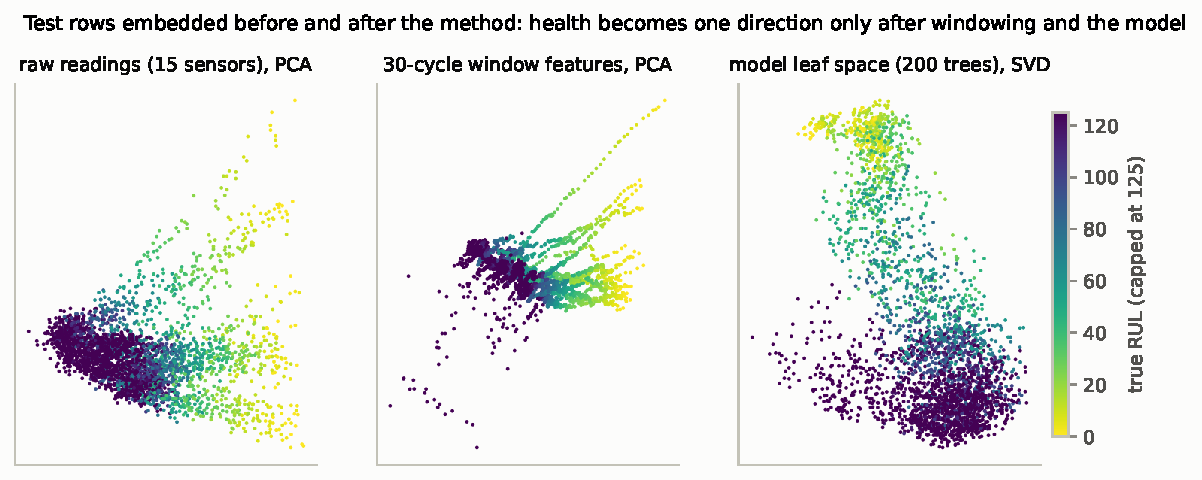
\includegraphics[width=\columnwidth]{embeddings.pdf}
\caption{Test rows embedded from raw readings, from window features, and from the model's leaf space, coloured by true RUL.}
\label{fig:emb}
\end{figure}

Of \EaTestRows{} test rows, \EaMisclassifiedRows{} (\EaMisclassifiedPct{}\%) get the wrong status, all between
neighbouring statuses. HEALTHY is never predicted CRITICAL, nor the reverse. The most frequent confusion is
WARNING predicted as HEALTHY (\EaTopConfusionRows{} rows). We inspected \EaInspected{} misclassified rows on
whole-engine plots: \EaAmbiguous{} are ambiguous, \EaMislabeled{} mislabeled (the labels are exact cycle counts),
and \EaModel{} are real model errors. These fall into four shapes. The prediction lags on engines that fail
fast (\EaPatternLagging{}) and runs early near the end of long-lived engines (\EaPatternEarly{}); both
regress toward the average degradation speed. Single-reading jitter accounts for \EaPatternJitter{}, and in
\EaPatternPlateau{} the tree output sticks near 60, on the WARNING line. Fig.~\ref{fig:emb} shows that health
becomes a single direction only after windowing and the model.

\section{Limitations}
FD001 is one simulated operating condition and fault mode; nothing here shows transfer to other conditions or
to real engines. Three seeds give a spread, not a confidence interval. The alert rule passes on every held-out
engine, but on all 100 engines it passes \AllEnginesAlertPass{}: a few training engines close a WARNING and
reopen it. Throughput was measured on one laptop with every component on it. The system was not deployed to a
cloud host.

\section{Conclusion}
A pre-registered test rejected the claim that the 8 top-ranked sensors suffice, and the service ships all 21.
The post hoc analysis changes what that rejection means. The ranking rule failed, not the idea of fewer sensors,
and a recipe choice of the same size as the effect means the verdict is conditional. As in other ML
systems~\cite{sculley2015}, the model was the small part. Most of the defects we caught were in the system
around it: a trend rule tuned for a clean signal, a double-counted score after restart, a window saved before
its score, and a test suite that leaked state into the dev Redis.

\bibliographystyle{IEEEtran}
\begin{thebibliography}{1}
\bibitem{saxena2008} A.~Saxena, K.~Goebel, D.~Simon, and N.~Eklund, ``Damage propagation modeling for aircraft engine run-to-failure simulation,'' in \emph{Proc. Int. Conf. Prognostics and Health Management (PHM)}, 2008.
\bibitem{heimes2008} F.~O.~Heimes, ``Recurrent neural networks for remaining useful life estimation,'' in \emph{Proc. Int. Conf. Prognostics and Health Management (PHM)}, 2008.
\bibitem{kreps2011} J.~Kreps, N.~Narkhede, and J.~Rao, ``Kafka: a distributed messaging system for log processing,'' in \emph{Proc. NetDB Workshop}, 2011.
\bibitem{pelkonen2015} T.~Pelkonen \emph{et al.}, ``Gorilla: a fast, scalable, in-memory time series database,'' \emph{Proc. VLDB Endowment}, vol.~8, no.~12, 2015.
\bibitem{sculley2015} D.~Sculley \emph{et al.}, ``Hidden technical debt in machine learning systems,'' in \emph{Advances in Neural Information Processing Systems (NeurIPS)}, 2015.
\end{thebibliography}

\end{document}
